\chapter{Progettazione Concettuale}

\section{Premesse alla lettura dei diagrammi}

\subsection{Modelli Utilizzati}

Procediamo alla modellizzazione del mini-mondo, partendo dalla progettazione concettuale.

Questa fase di progettazione è stata svolta utilizzando, oltre che il modello \textbf{UML} nella forma di un \textbf{Class Diagram}, anche il modello \textbf{EER}, ovvero \textbf{Enhanced Entity Relationship}, per cogliere meglio aspetti del dominio che un modello \textbf{ER} classico non avrebbe potuto cogliere, come ad esempio \textbf{generalizzazioni e specializzazioni}.

\subsection{Precisazioni sui Diagrammi}

\subsubsection{EER Diagram}

Vista la densità del diagramma \textbf{EER}, si è deciso d'introdurre un \textbf{color coding} per facilitarne la lettura:

\begin{itemize}
  \item \textcolor{PRIMARY}{Entità}, e dunque Specializzazioni in \textcolor{PRIMARY}{arancione};
  \item \textcolor{CONTRAST}{Relazioni} in \textcolor{CONTRAST}{celeste};
  \item \textcolor{NEWGREEN}{Attributi} in \textcolor{NEWGREEN}{verde};
\end{itemize}

Inoltre, in caso di accavallamento di linee, si è deciso d'interrompere la linea in secondo piano in corrispondenza di un intersezione, così da evidenziare i diversi collegamenti.

\subsubsection{UML Class Diagram}

Per migliorare la leggibilità dei diagrammi, si è deciso di specificare le \textbf{molteplicità} degli attributi esclusivamente per sottolineare la possibilità di essere valorizzato a \textbf{NULL}. 

In tali casi si è utilizzata la molteplicità \textbf{[\(0..1\)]} esclusivamente per gli attributi di tipo \textbf{Bool}, mentre \textbf{[\(0..*\)]} per gli altri.

\bigskip

\begin{note}[Leggibilità dei Diagrammi]
  In caso di problemi di leggibilità dei diagrammi, sono disponibili le versioni originali nella pagina GitHub del progetto:
  \exlink{https://github.com/RiccardoElena/UninaDelivery/blob/develop/db/docs/sources/ER_Diagram.pdf}{ER Diagram} e \exlink{https://github.com/RiccardoElena/UninaDelivery/blob/develop/db/docs/sources/UML_Class_Diagram.pdf}{UML Class Diagram}.
\end{note}

\newpage

\section{Enhanced Entity Relationship Diagram}
\begin{center}
  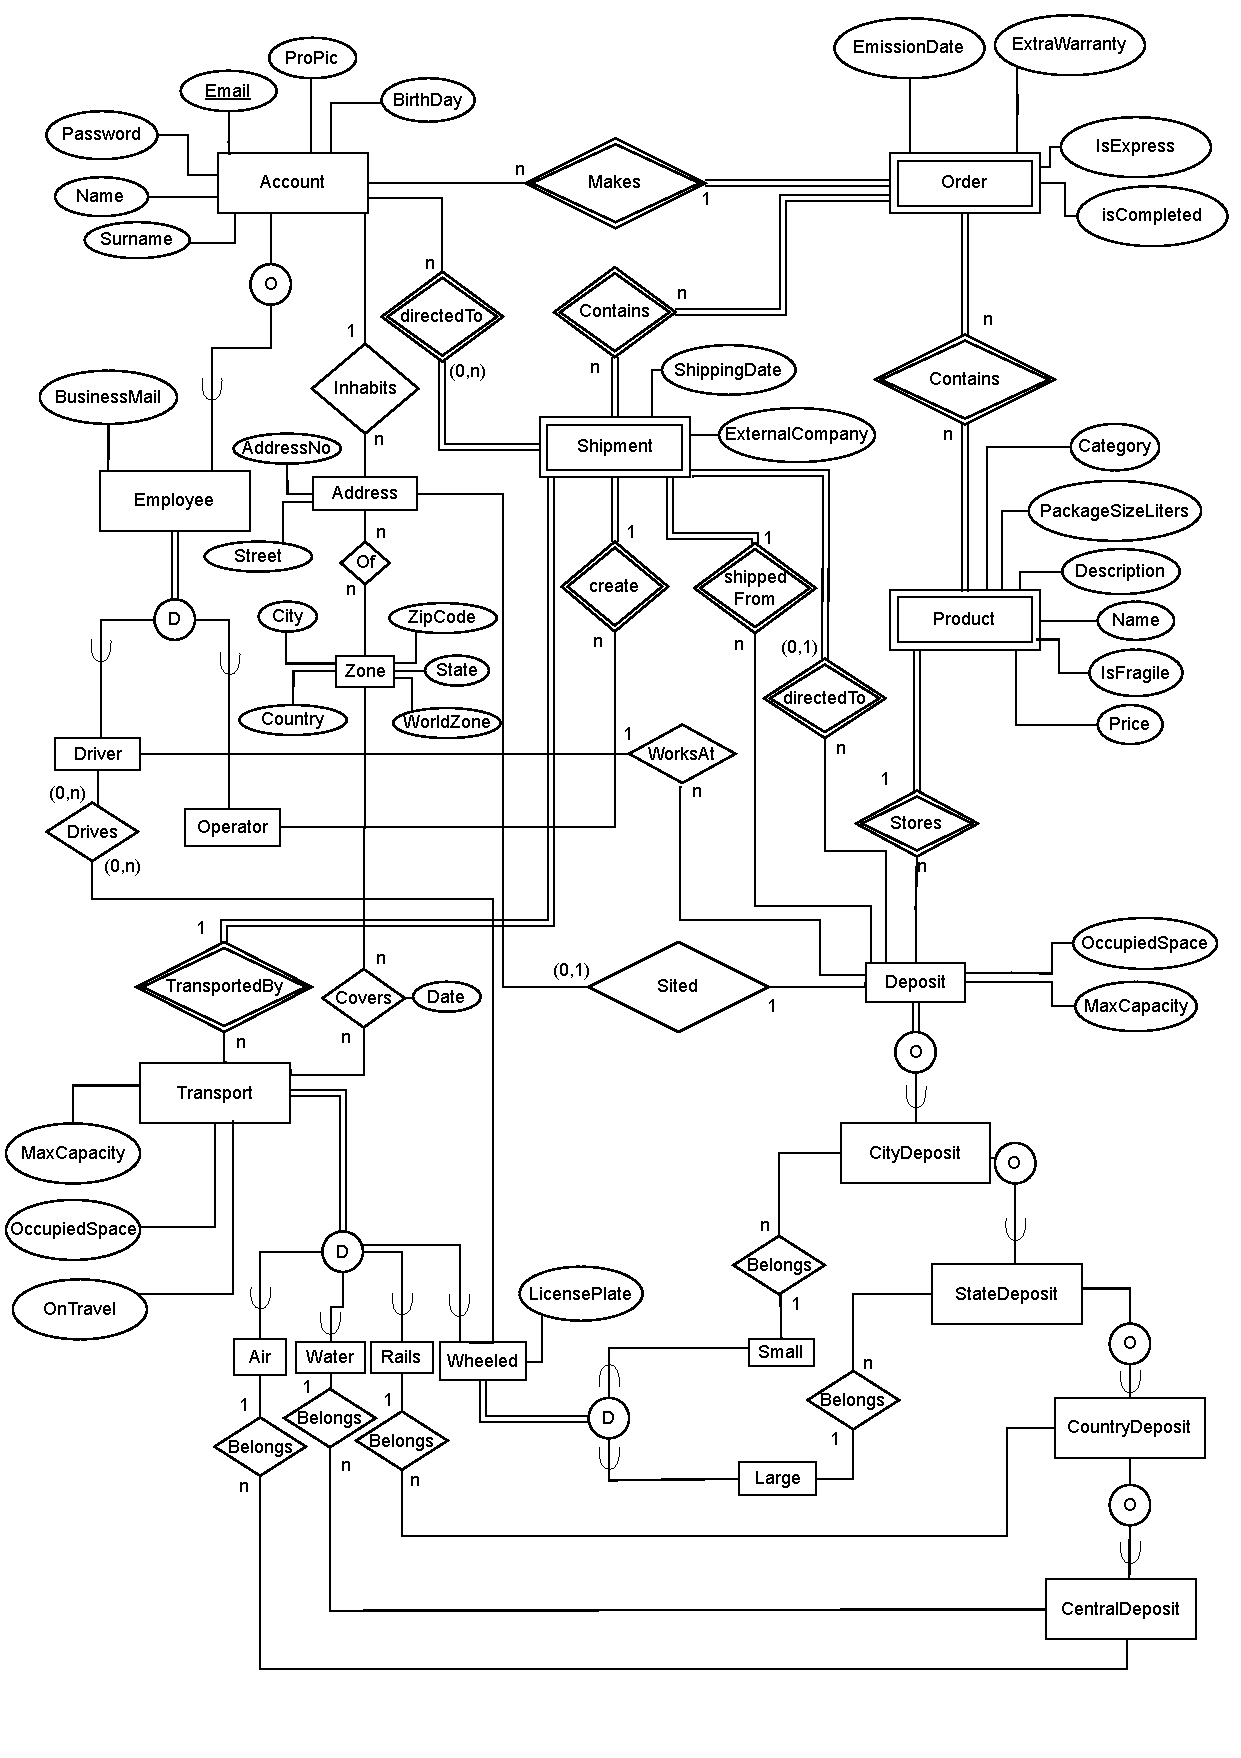
\includegraphics[width=0.9\textwidth]{ER_Diagram.pdf}
\end{center}

\section{UML Class Diagram}
\begin{center}
  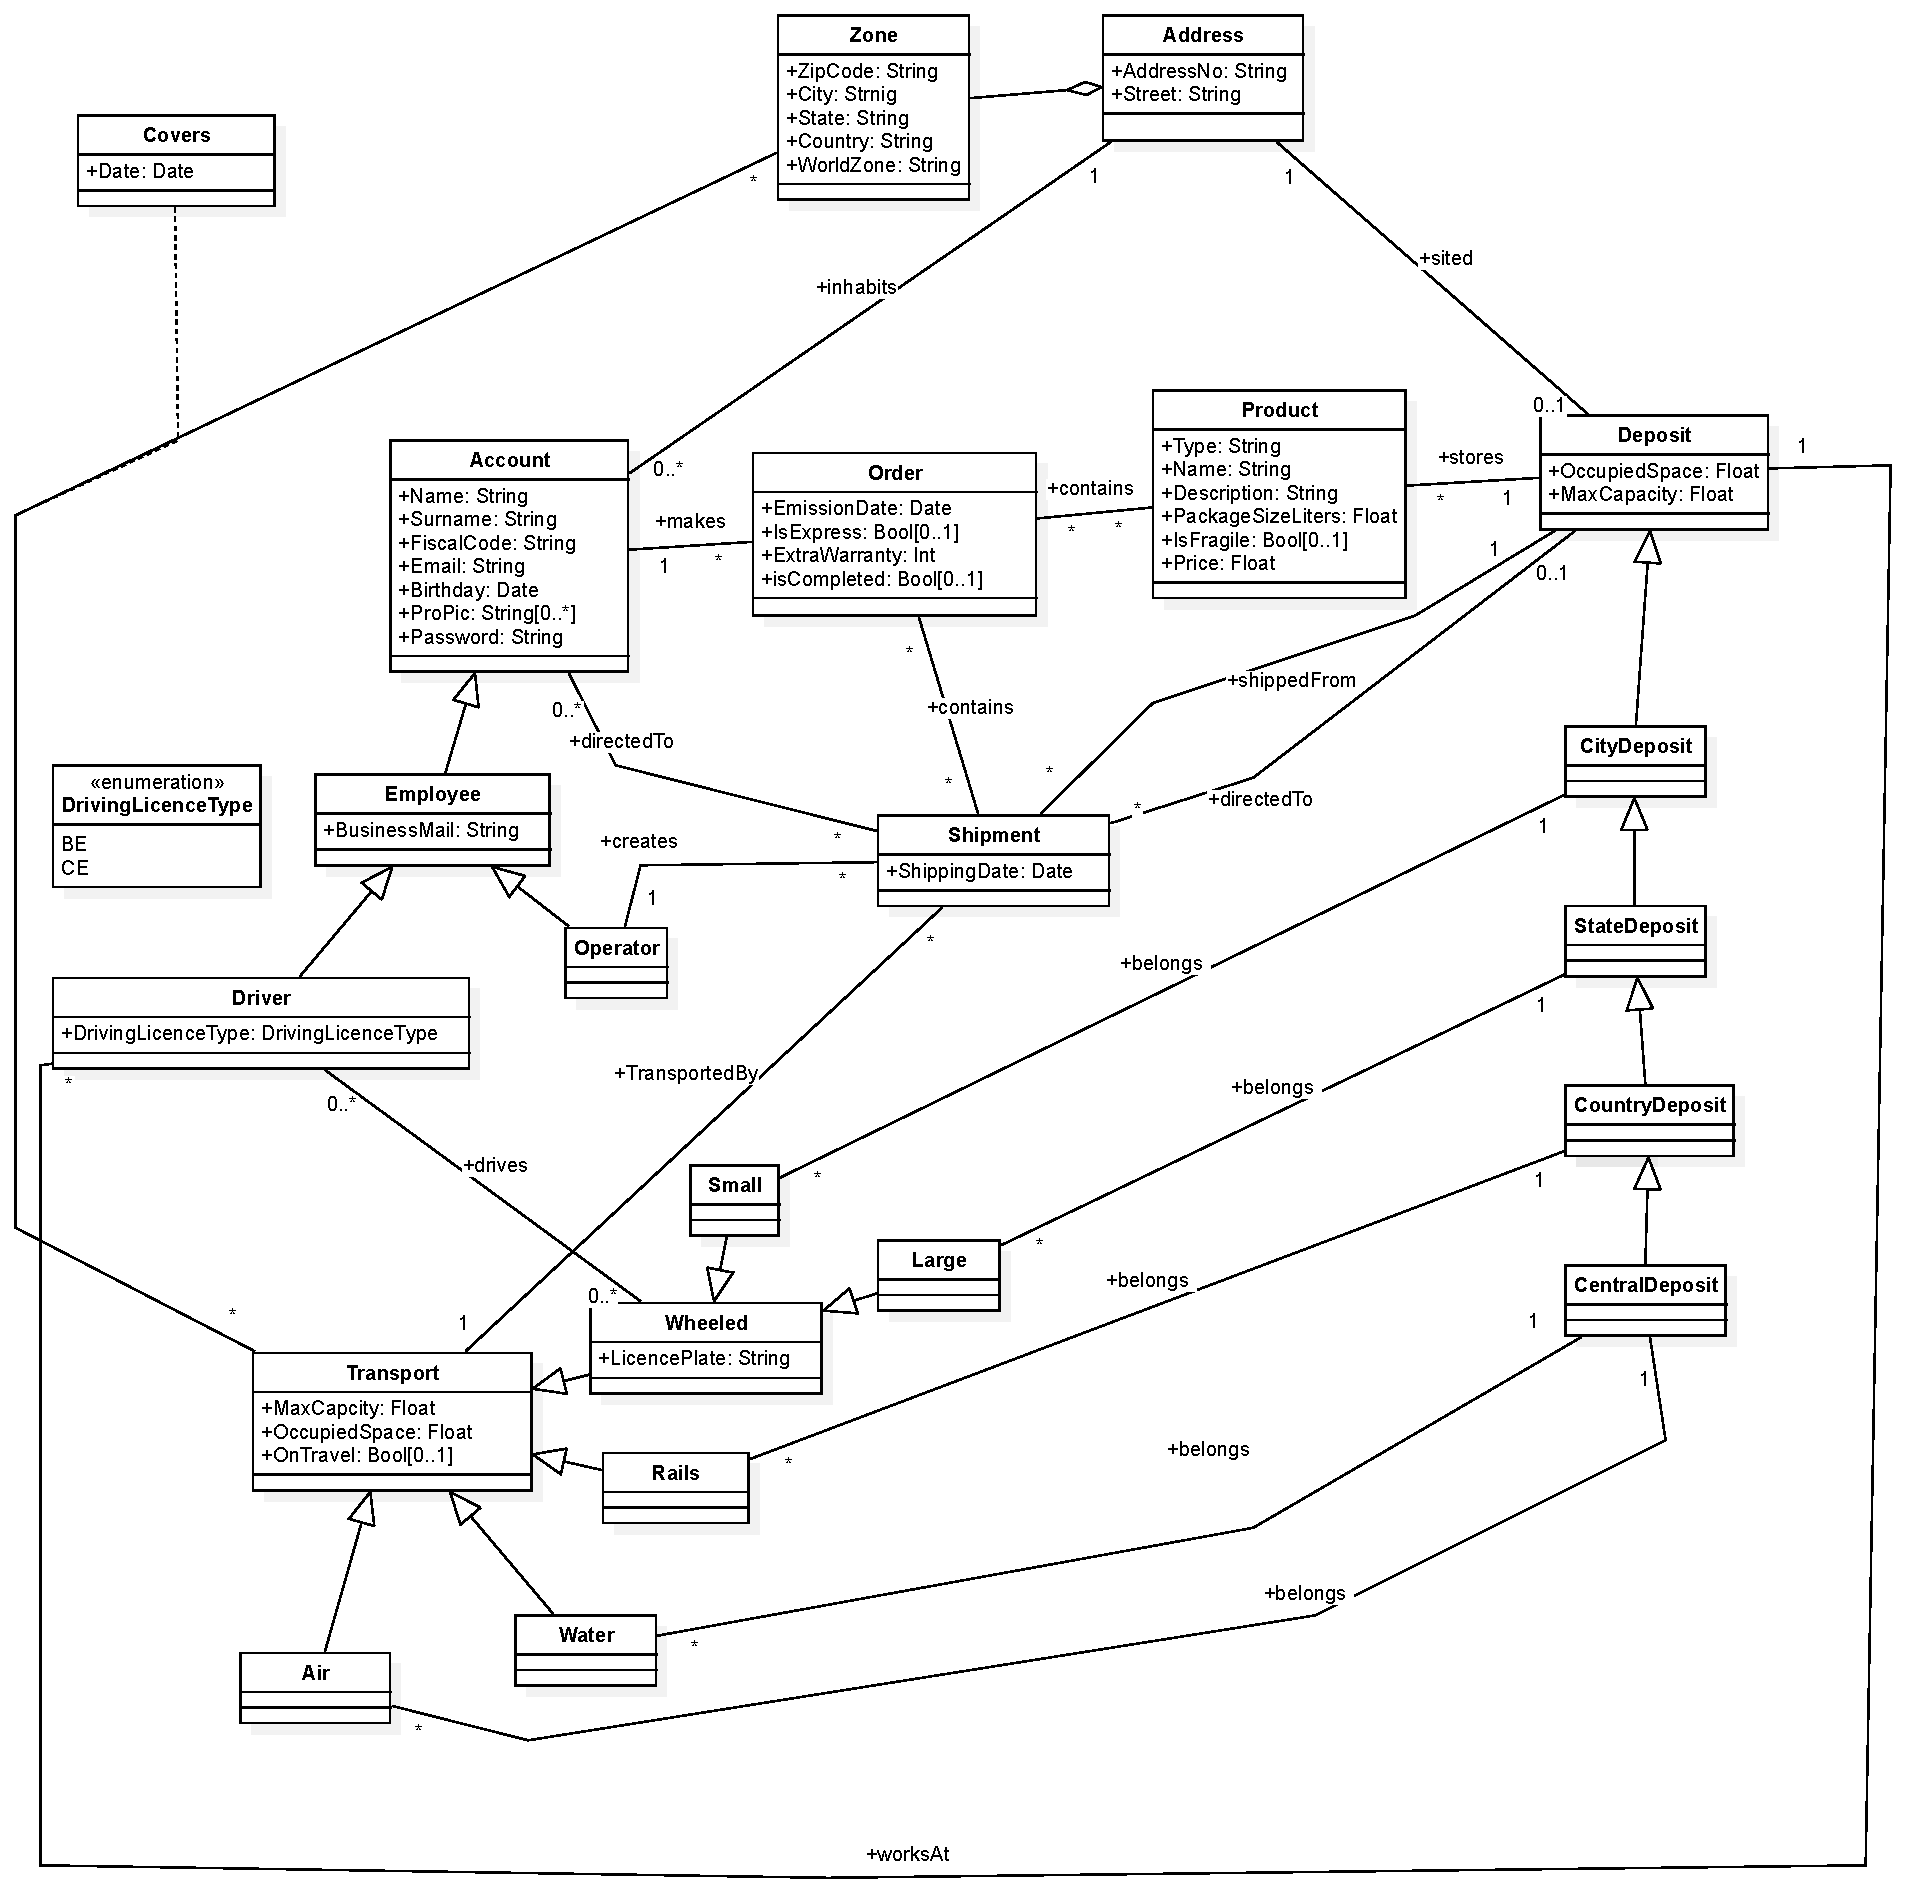
\includegraphics[width=\textwidth]{UML_Class_Diagram.pdf}
\end{center}

\newpage

\section{Ristrutturazione del Diagramma UML}
% TODO @zGenny 
% [ ] populate the db and play around with it to see if everything works as expected. You can try violating the constraint in the dictonary and see if the db blocks you
\subsection{Considerazioni sulla Ristrutturazione}

\subsubsection{Attributi Multipli e Multivalore}

Nello schema concettuale non sono presenti attributi \textbf{Multipli} o \textbf{Multivalore}, in quanto non sono stati ritenuti necessari per la rappresentazione del mini-mondo.

\subsubsection{Attributi Derivati}

Nello schema concettuale sono presenti due attributi \textbf{Derivati}:

\begin{itemize}
  \item L'attributo \textbf{Price} dell'entità \textbf{Shipment}, il quale però non ha necessità di essere conservato, non essendo un attributo di frequente richiesta per il sistema richiesto, e che quindi può essere eventualmente calcolato \textit{on-the-fly} in fase d'interrogazione del database basandosi sugli indirizzi di partenza e arrivo della spedizione e sulle eventuali modalità extra di consegna specificate in \textbf{Order}, come \textit{ExtraWarranty} e \textit{IsExpress}.
  \item L'attributo \textbf{IsCompleted} dell'entità \textbf{Order}, invece, si è scelto di conservarlo, in quanto è un attributo che può essere richiesto frequentemente dal sistema, e richiede un controllo relativamente complesso per essere valorizzato. Un ordine è considerato \textit{completato} se tutti i prodotti che contiene sono stati consegnati all'utente, dunque sarebbe necessario infatti controllare che tutti i prodotti dell'ordine siano stati spediti al destinatario, e che tali spedizioni siano andate a buon fine, coinvolgendo ben quattro entità: \textbf{Order}, \textbf{Product}, \textbf{Shipment} e \textbf{Account}. % * We should add a trigger that does this the first time
  \item L'attributo \textbf{OccupiedSpace} sia dell'entità \textbf{Deposit} che dell'entità \textbf{Transport}, infine, è stato anch'esso conservato, in quanto è un attributo che può essere richiesto frequentemente dal sistema, e richiede un interrogazione con risultato potenzialmente molto grande per essere valorizzata. % * this can be a cool trigger too.
\end{itemize}

\subsubsection{Generalizzazioni e Specializzazioni}

Le varie \textbf{Generalizzazioni} e \textbf{Specializzazioni} presenti nello schema concettuale sono state ristrutturate usando metodologie diverse, in base alla loro natura.

\begin{itemize}
  \item[\textbf{Employee:}] Essendo la specializzazione \textbf{Totale Disgiunta}, ed essendo le classi coinvolte in poche associazioni, si è scelto di accorpare la classe generale in quelle specializzate.
  \item[\textbf{Account:}] Essendo la specializzazione \textbf{Parziale Overlapping}, si è deciso di trasformarla in \textbf{Associazione}, limitando così il più possibile il numero di campi \textbf{NULL} e di \textbf{Vincoli d'Integrità}.
  \item[\textbf{Deposit:}] In questo caso trattandosi di una gerarchia di specializzazione si è scelto di accorpare a cascata le classi specializzate in quella generale, non avendo le classi specializzate attributi ed essendo tutte coinvolte in un'unica associazione concettualmente identica che verrà successivamente analizzata.
  \item[\textbf{Transport:}] Analogamente a quanto visto per \textbf{Deposit}, nonostante non si tratti di una gerarchia, si è scelto di accorpare le classi specializzate in quella generale. 
\end{itemize}

\subsubsection{Analisi delle Ridondanze}\label{Redundancy analysis}

Vediamo infine le ridondanze presenti nello schema concettuale, e come sono state rimosse.

Dalla ristrutturazione delle \textbf{Specializzazioni} di \textbf{Transport} sono emersi quattro attributi che servono essenzialmente lo stesso scopo ma per tipologie diverse di mezzi di trasporto: \textbf{Licence Plate}, \textbf{TrainNo}, \textbf{IMOCode} e \textbf{FlightNo}. Si è quindi deciso di accorpare questi attributi in un unico attributo \textbf{TransportID}, che può essere valorizzato con un identificativo univoco condiviso tra le tipologie di mezzi di trasporto, eliminando la possibilità di valori \textbf{NULL} o di valori uguali per tipi di mezzi diversi che imponevano aggiunta di vincoli o presenza di più attributi.

Inoltre la ristrutturazione delle \textbf{Specializzazioni} di \textbf{Deposit} ha fatto emergere quattro associazioni identiche a meno di vincoli che le riguardano, ovvero le associazioni \textbf{belongs}. È possibile dunque ridurle a un'unica associazione preservando i vincoli.

In ultima analisi, la classe \textbf{Shipment} è coinvolta in due associazioni semanticamente identiche, che si distinguono solo per molteplicità e seconda classe coinvolta, ovvero \textbf{Account} e \textbf{Deposit}. In particolare quella con \textbf{Account} è un'associazione circolare, essendo entrambe le classi associate anche con \textbf{Order}. Si è quindi deciso di eliminare l'associazione con \textbf{Account}, essendo il destinatario della spedizione già noto tramite \textbf{Order}.

\subsection{Identificazione delle Chiavi primarie}\label{individuazioneDelleChiaviPrimarie}

Aldilà delle chiavi primarie già presenti nello schema concettuale esplicitate nel \textbf{diagramma ER} e dell'attributo \textbf{TransportID} introdotto \intlink{Redundancy analysis}{precedentemente}, si è deciso di aggiungere chiavi surrogate per le entità \textbf{Order}, \textbf{Shipment} e \textbf{Deposit}, poiché migrando le chiavi di altre entità si sarebbero ottenute chiavi composte troppo lunghe e complesse.

Per l'entità \textbf{Address} invece, è risultato più appropriato migrare la chiave primaria di \textbf{Area} essendo una composizione e di conseguenza già concettualmente una \textit{parte} dell'entità \textbf{Address}. 

\newpage

\subsection{Class Diagram Ristrutturato}

\begin{center}
  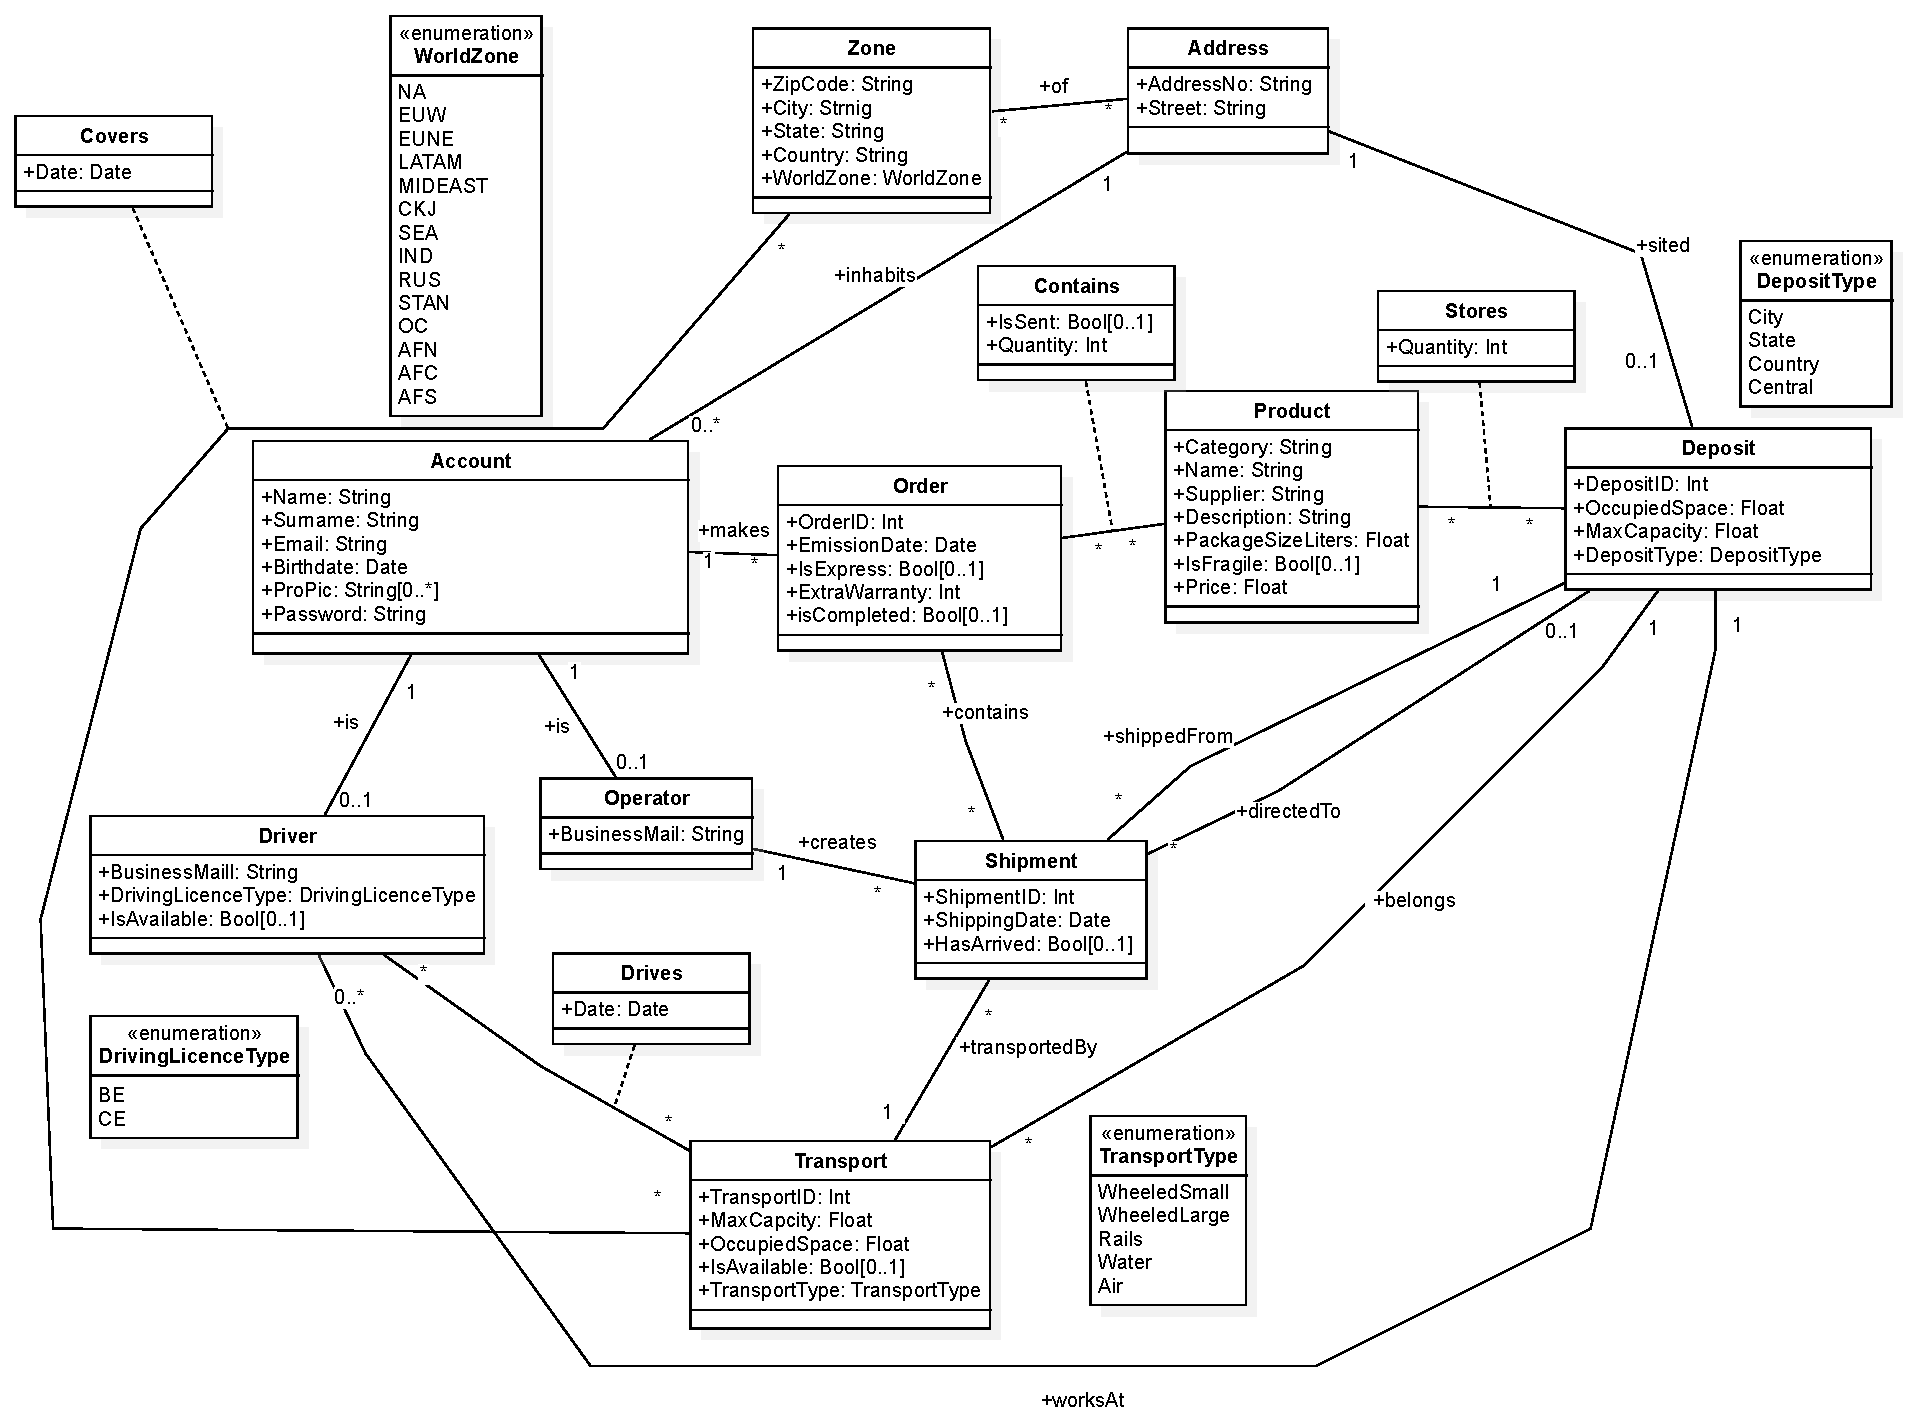
\includegraphics[width=\textwidth]{UML_Class_Diagram_Restructured.pdf} 
\end{center}

\newpage

\section{Dizionari}

\subsection{Dizionario delle Classi}

\customTable{cYY}[Dizionario delle classi Prima Parte]{\textbfB{Classe} & \textbfB{Descrizione} & \textbfB{Attributi}}{
  \textbf{Account} & Generico utente che utilizza il sistema per effettuare ordini. & 
  {\footnotesize 
  \textbf{Name:} (\textit{string}): Nome dell'utente;
  
  \textbf{Surname} (\textit{string}): Cognome dell'utente;
  
  \textbf{Email} (\textit{string}): Chiave Primaria. Email dell'utente;

  \textbf{Birthdate} (\textit{date}): Data di nascita dell'utente;

  \textbf{ProPic} (\textit{string}): Eventuale immagine profilo dell'utente;

  \textbf{Password} (\textit{string}): Password dell'utente;  
  }\\


  \textbf{Operator} & Account di un impiegato che si occupa di creare le spedizioni. &
  {\footnotesize
  \textbf{BusinessMail} (\textit{string}): Chiave Primaria. Email aziendale dell'operatore;
  }\\


  \textbf{Driver} & Account di un autista che si occupa di effettuare le consegne. &
  {\footnotesize
  \textbf{BusinessMail} (\textit{string}): Chiave Primaria. Email aziendale dell'autista;

  \textbf{DrivingLincenceType} (\textit{DrivingLincenceType}): Tipologia di patente dell'autista;

  \textbf{IsAvailable} (\textit{bool}): Indica se l'autista è disponibile o meno;
  }\\


  \textbf{Order} & Ordine effettuato da un utente. Può contenere più prodotti e può essere spedito in più spedizioni. &
  {\footnotesize
  \textbf{OrderID} (\textit{integer}): Chiave Surrogata. Identificativo dell'ordine;

  \textbf{EmissionDate} (\textit{date}): Data di emissione dell'ordine;

  \textbf{IsExpress} (\textit{bool}): Indica se l'ordine è espresso o meno;

  \textbf{ExtraWarranty} (\textit{bool}): Indica se è stata acquistata una garanzia extra o meno;

  \textbf{IsCompleted} (\textit{bool}): Indica se l'ordine è stato completato o meno;
  }\\


  \textbf{Shipment} & Singola spedizione partita da un deposito. Può contenere più ordini e può raggiungere a più utenti o a un deposito. &
  {\footnotesize
  \textbf{ShipmentID} (\textit{integer}): Chiave Surrogata. Identificativo della spedizione; 

  \textbf{ShippingDate} (\textit{date}): Data della spedizione;
  }\\  
}

\newpage

\customTable{cYY}[Dizionario delle classi Seconda Parte]{\textbfB{Classe} & \textbfB{Descrizione} & \textbfB{Attributi}}{
  \textbf{Product} & Prodotto acquistabile da un utente. Può essere conservato in più depositi. &
  { \footnotesize
    \textbf{Type} (\textit{string}): Categoria del prodotto;

    \textbf{Name} (\textit{string}): Chiave Primaria. Nome del prodotto;

    \textbf{Supplier} (\textit{string}): Chiave Primaria. Fornitore del prodotto. Di default è \textit{UninaDelivery};
  
    \textbf{Description} (\textit{string}): Descrizione del prodotto;

    \textbf{PackageSizeLiters} (\textit{float}): Dimensione del prodotto in litri;

    \textbf{IsFagile} (\textit{bool}): Indica se il prodotto è fragile o meno;

    \textbf{Price} (\textit{float}): Prezzo del prodotto;
  }\\


  \textbf{Deposit} & Deposito per la conservazione di prodotti. Può contenere più prodotti e può essere raggiunto da più spedizioni. &
  {\footnotesize
  \textbf{DepositID} (\textit{integer}): Chiave Surrogata. Identificativo del deposito;

  \textbf{OccupiedSpace} (\textit{float}): Spazio del deposito attualmente occupato;

  \textbf{MaxCapacity} (\textit{float}): Spazio massimo del deposito;

  \textbf{DepositType} (\textit{DepositType}): Tipologia del deposito;
  }\\
  

  \textbf{Area} & Zona del mondo raggiungibile da un mezzo di trasporto. Contiene più indirizzi. &
  {\footnotesize
  \textbf{ZipCode} (\textit{string}): Chiave Primaria. Codice di Avviamento Postale della zona;

  \textbf{City} (\textit{string}): Città in cui si trova la zona;

  \textbf{Country} (\textit{string}): Chiave Primaria. Paese in cui si trova la zona;
  
  \textbf{WorldZone} (\textit{string}): Zona del mondo in cui si trova la zona;
  }\\

  \textbf{Address} & Indirizzo di un utente o di un deposito. & 
  {\footnotesize

  \textbf{AddressNo} (\textit{string}): Chiave Primaria. Numero civico dell'indirizzo; 

  \textbf{Street} (\textit{string}): Via dell'indirizzo;
  }\\

  \textbf{Transport} & Mezzo di trasporto utilizzato per le spedizioni. & 
  {\footnotesize
  \textbf{TransportID} (\textit{integer}): Chiave Surrogata. Identificativo del mezzo di trasporto;

  \textbf{MaxCapacity} (\textit{float}): Capacità massima del mezzo di trasporto;

  \textbf{OccupiedSpace} (\textit{float}): Spazio attualmente occupato dal mezzo di trasporto;

  \textbf{IsAvailable} (\textit{bool}): Indica se il mezzo di trasporto è disponibile o meno. Il campo sarà valorizzato a \textit{true} solo se il mezzo non è già in viaggio;
  
  \textbf{TransportType} (\textit{TransportType}): Tipologia del mezzo di trasporto;
  }\\

}

\subsection{Dizionario delle Associazioni}

\customTable{cYYY}[Dizionario delle associazioni Prima Parte]{\textbfB{Associazione} & \textbfB{Descrizione} & \textbfB{Attributi} & \textbfB{Classi Coinvolte}}{
  \textbf{Makes} & 
  {\footnotesize
  Esprime la relazione tra un \textbf{Account} e un \textbf{Order}. Un \textbf{Account} può effettuare più \textbf{Order}, mentre un \textbf{Order} è effettuato da un solo \textbf{Account}.
  } & 
  --- & 
  {\footnotesize
  \textbf{Account \([1]\)} (\textit{makes}): L'account che effettua un dato ordine;

  \textbf{Order \([*]\)} (\textit{made by}): Gli ordini effettuati da un dato account;
  
  }\\

  \textbf{Inhabits} &
  {\footnotesize
  Esprime la relazione tra un \textbf{Account} e un \textbf{Address}. Un \textbf{Account} può avere un solo \textbf{Address}, mentre un \textbf{Address} può corrispondere a più \textbf{Account}.
  } &
  --- &
  {\footnotesize
  \textbf{Account \([0..*]\)} (\textit{inhabits}): Gli account che abitano in un dato indirizzo;

  \textbf{Address \([1]\)} (\textit{is inhabited by}): L'indirizzo abitato da un dato account;
  }\\

  \textbf{Sited} &
  {\footnotesize
  Esprime la relazione tra un \textbf{Address} e un \textbf{Deposito}. Un \textbf{Address} può corrispondere a un solo \textbf{Deposit}, mentre un \textbf{Deposit} ha solo un \textbf{Address}.
  } &
  --- &
  {\footnotesize
  \textbf{Address \([1]\)} (\textit{is site of}): L'indirizzo di un dato deposito;

  \textbf{Deposit \([1]\)} (\textit{sited on}): Il deposito che si trova in un dato indirizzo;
  
  }\\
  
  \textbf{Located} &
  {\footnotesize
  Esprime la relazione tra \textbf{Area} e \textbf{Address}. Un \textbf{Area} può contenere più \textbf{Address}, e un \textbf{Address} appartiene a un'unica \textbf{Area}.
  } &
  --- &
  {\footnotesize
  \textbf{Area \([*]\)} (\textit{is location}): Le Area che contengono un dato indirizzo;

  \textbf{Address \([*]\)} (\textit{located}): Gli indirizzi che appartengono a una data zona;
  }\\

  \textbf{Contains} &
  {\footnotesize
  Esprime la relazione tra \textbf{Order} e \textbf{Product}. Un \textbf{Order} può contenere una quantità N di \textbf{Product} e un \textbf{Product} può essere contenuto in più \textbf{Order}. 
  } &
  --- 
  &
  {\footnotesize
  \textbf{Order \([*]\)} (\textit{contains}): Gli ordini che contengono un dato prodotto;

  \textbf{Product \([1]\)} (\textit{is contained}): Il prodotto contenuto in un dato ordine;
  }\\
}
\customTable{cYYY}[Dizionario delle associazioni Seconda Parte]{\textbfB{Associazione} & \textbfB{Descrizione} & \textbfB{Attributi} & \textbfB{Classi Coinvolte}}{
  \textbf{Stores} &
  {\footnotesize
  Esprime la relazione tra \textbf{Deposit} e \textbf{Product}. Un \textbf{Deposit} può contenere più \textbf{Product}, mentre un \textbf{Product} può essere contenuto in più \textbf{Deposit}.
  } &
  {\footnotesize

  \textbf{Quantity} (\textit{integer}): Numero di pezzi di un dato prodotto conservati in un deposito; 
  } &
  
  {\footnotesize
  \textbf{Deposit \([*]\)} (\textit{stores}): I depositi che contengono un dato prodotto;

  \textbf{Product \([*]\)} (\textit{is stored in}): I prodotti contenuti in un dato deposito;
  
  }\\

  \textbf{ShippedFrom} &
  {\footnotesize
  Esprime la relazione tra \textbf{Shipment} e \textbf{Deposit} \textit{mittente}. Una \textbf{Shipment} può avere un solo mittente, mentre un \textbf{Deposit} può essere mittente di più \textbf{Shipment}.
  } &
  --- &
  {\footnotesize
  \textbf{Shipment \([*]\)} (\textit{shipped}): Le spedizioni che partono da un dato deposito; 

  \textbf{Deposit \([1]\)} (\textit{seder}): Il deposito mittente di una data spedizione; 
  }\\
  
  \textbf{Ships} &
  {\footnotesize
  Esprime la relazione tra \textbf{Shipment} e \textbf{Order}. Una \textbf{Shipment} può contenere più \textbf{Order}, mentre un \textbf{Order} può essere contenuto in più \textbf{Shipment}.
  } &
  --- &
  {\footnotesize
  \textbf{Shipment \([*]\)} (\textit{ships}): Le spedizioni che spediscono un dato ordine; 

  \textbf{Order \([*]\)} (\textit{is shipped}): Gli ordini spediti da una data spedizione; 
  }\\

  \textbf{Creates} &
  {\footnotesize
  Esprime la relazione tra l'\textbf{Operator} e l'\textbf{Order}. Un \textbf{Operator} può creare più \textbf{Order}, mentre un \textbf{Order} può essere creato da un solo \textbf{Operator}.
  } &
  --- &
  {\footnotesize
  \textbf{Operator \([1]\)} (\textit{creates}): L'operatore che crea una data spedizione; 

  \textbf{Shipment \([*]\)} (\textit{is created}): Le spedizioni create da un dato operatore; 
  }\\

  \textbf{TransportedBy} &
  {\footnotesize
  Esprime la relazione tra \textbf{Shipment} e \textbf{Transport}. Una \textbf{Shipment} può essere trasportata da un solo \textbf{Transport}, mentre un \textbf{Transport} può trasportare più \textbf{Shipment}.
  } &
  --- &
  {\footnotesize
  \textbf{Shipment \([*]\)} (\textit{transported by}): Le spedizioni trasportate da un dato mezzo di trasporto;; 

  \textbf{Transport \([1]\)} (\textit{transports}): Il mezzo di trasporto che trasporta una data spedizione; 
  }\\
  
}
\customTable{cYYY}[Dizionario delle associazioni Terza Parte]{\textbfB{Associazione} & \textbfB{Descrizione} & \textbfB{Attributi} & \textbfB{Classi Coinvolte}}{
  
  \textbf{Belongs} &
  {\footnotesize
  Esprime la relazione tra \textbf{Transport} e \textbf{Deposit}. Un \textbf{Transport} può appartenere a un solo \textbf{Deposit}, mentre un \textbf{Deposit} può avere più \textbf{Transport}.
  } &
  --- &
  {\footnotesize
  \textbf{Deposit \([1]\)} (\textit{is belonged}): Il deposito a cui appartiene un dato mezzo di trasporto; 

  \textbf{Transport \([*]\)} (\textit{belongs}): I mezzi di trasporto che appartengono a un dato deposito; 
  }\\

  \textbf{Is} &
  {\footnotesize
  Esprime la relazione tra \textbf{Account} e \textbf{Driver}. Indica se un \textbf{Account} oltre a essere un cliente è anche un \textbf{Driver}.
  } &
  --- &
  {\footnotesize
  \textbf{Account \([1]\)} (\textit{is}): I dati generali dell'account di un dato autista; 

  \textbf{Driver \([0..1]\)} (\textit{has}): I dati specifici dell'autista di un dato account;
  }\\

  \textbf{Is} &
  {\footnotesize
  Esprime la relazione tra \textbf{Account} e \textbf{Operator}. Indica se un \textbf{Account} oltre a essere un cliente è anche un \textbf{Operator}.
  } &
  --- &
  {\footnotesize
  \textbf{Account \([1]\)} (\textit{is}): I dati generali dell'account di un dato operatore; 

  \textbf{Operator \([0..1]\)} (\textit{has}): I dati specifici dell'operatore di un dato account;
  }\\

  \textbf{WorksAt} &
  {\footnotesize
  Esprime la relazione tra \textbf{Driver} e \textbf{Deposit}. Un \textbf{Driver} può lavorare in un solo \textbf{Deposit}, mentre un \textbf{Deposit} può avere più \textbf{Driver}.
  } &
  --- &
  {\footnotesize
  \textbf{Driver \([0..*]\)} (\textit{works at}): Gli autisti che lavorano per un dato deposito; 

  \textbf{Deposit \([1]\)} (\textit{employs}): Il deposito che impiega un dato autista; 
  }\\

  \textbf{Covers} &
  {\footnotesize
  Esprime la relazione tra \textbf{Transport} e \textbf{Area}. Un \textbf{Transport} può coprire più \textbf{Area}, mentre una \textbf{Area} può essere coperta da più \textbf{Transport}.
  } &
  {\footnotesize

  \textbf{Date} (\textit{date}): Data in cui un trasporto copre una certa zona. Un trasporto non può coprire più Area nella stessa data; 
  
  } &
  {\footnotesize
  \textbf{Area \([*]\)} (\textit{is covered}): Le Area coperte da un dato mezzo di trasporto;

  \textbf{Transport \([*]\)} (\textit{covers}): I trasporti che coprono una data zona. Anche più di uno per data;
  }\\

  \textbf{Drives} &
  {\footnotesize
  Esprime la relazione tra \textbf{Driver} e \textbf{Transport}. Un \textbf{Driver} può guidare più \textbf{Transport}, mentre un \textbf{Transport} può essere guidato da più \textbf{Driver}.
  
  } &
  {\footnotesize

  \textbf{Date} (\textit{date}): Data in cui un autista giuda un mezzo di trasporto. Un trasporto non può essere guidato da più autisti nella stessa data e viceversa; 
  
  } &
  {\footnotesize
  \textbf{Driver \([*]\)} (\textit{drives}): Gli autisti che guidano per un dato mezzo di trasporto; 
  \textbf{Transport \([*]\)} (\textit{is driven}): I mezzi di trasporto guidati da un dato autista;
  }\\
}

\subsection{Dizionario dei Vincoli}

\customTable{ccY}[Dizionario dei vincoli Prima Parte]{\textbfB{Vincolo} & \textbfB{Tipologia} & \textbfB{Descrizione}}{
  \textbf{formatAccountName} & Dominio &
  {\footnotesize
  Il campo \textbf{Name} della classe \textbf{Account} deve contenere solo caratteri alfabetici
  }\\

  \textbf{formatAccountSurname} & Dominio &
  {\footnotesize
  Il campo \textbf{Surname} della classe \textbf{Account} deve contenere solo caratteri alfabetici
  }\\

  \textbf{formatAccountEmail} & Dominio &
  {\footnotesize
  Il campo \textbf{Email} della classe \textbf{Account} deve avere il formato `\textbf{word}@\textbf{domain}.\textbf{ext}', dove \textit{word} può contenere solo caratteri alfanumerici o al più dei punti, \textit{domain} da soli caratteri alfabetici o punti, mentre \textit{ext} da solo caratteri alfabetici, e dev'essere lunga almeno due caratteri.
  }\\

  \textbf{validOperatorBusinessmail} & Dominio &
  {\footnotesize
  Il campo \textbf{Businessmail} della classe \textbf{Operator} deve avere il formato `\textbf{word}@\textbf{domain}.\textbf{ext}', dove \textit{word} può contenere solo caratteri alfanumerici o al più dei punti, \textit{domain} da soli caratteri alfabetici o punti, mentre \textit{ext} da solo caratteri alfabetici, e dev'essere lunga almeno due caratteri.
  }\\

  \textbf{validDriverBusinessmail} & Dominio &
  {\footnotesize
  Il campo \textbf{Businessmail} della classe \textbf{Driver} deve avere il formato `\textbf{word}@\textbf{domain}.\textbf{ext}', dove \textit{word} può contenere solo caratteri alfanumerici o al più dei punti, \textit{domain} da soli caratteri alfabetici o punti, mentre \textit{ext} da solo caratteri alfabetici, e dev'essere lunga almeno due caratteri.
  }\\
  
  \textbf{validAccountBirthdate} & Dominio & 
  {\footnotesize
  L'utente deve aver compiuto 16 anni
  }\\

  \textbf{formatAccountProPic} & Dominio &
  {\footnotesize
  Il campo \textbf{ProPic} deve essere una stringa in formato \textit{Base64} compatibile con un immagine in formato `JPEG'. 
  }\\

  \textbf{formatAccountPassword} & Dominio &
  {\footnotesize
  Il campo \textbf{Password} della classe \textbf{Account} dev'essere una valida stringa codificata dall'algoritmo HASH SHA-256.
  }\\

}

\customTable{ccY}[Dizionario dei vincoli Seconda Parte]{\textbfB{Vincolo} & \textbfB{Tipologia} & \textbfB{Descrizione}}{

  \textbf{formatTransportMaxCapacity} & Dominio &
  {\footnotesize
  Il campo \textbf{MaxCapacity} della classe \textbf{Transport} dev'essere positivo.
  }\\

  \textbf{formatTransportOccupiedSpace} & Dominio &
  {\footnotesize
  Il campo \textbf{OccupiedSpace} della classe \textbf{Transport} dev'essere non negativo.
  }\\

  \textbf{formatOrderExtraWarranty} & Dominio &
  {\footnotesize
  Il campo \textbf{ExtraWarranty} della classe \textbf{Order} deve essere non negativo.
  }\\

  \textbf{formatOrderEmissionDate} & Dominio &
  {\footnotesize
    Il campo \textbf{EmissionDate} della classe \textbf{Order} non può essere successiva alla data corrente.
  }\\

  \textbf{formatAddressAddressNo} & Dominio &
  {\footnotesize
  Il campo \textbf{AddressNo} della classe \textbf{Address} dev'essere una stringa formata da sole cifre, seguita al più da una lettera, eventualmente seguita dalla parola `BIS'.
  }\\
  \textbf{formatAddressStreet} & Dominio &
  {\footnotesize
  Il campo \textbf{Street} della classe \textbf{Address} può contenere solo caratteri alfanumerici o al più il carattere \textit{`.'}.
  }\\
  
  \textbf{formatDepositOccupiedSpace} & Dominio & 
  {\footnotesize
  Il campo \textbf{OccupiedSpace} della classe \textbf{Deposit} deve essere un float non negativo.
  }\\
  
  \textbf{formatDepositMaxCapacity} & Dominio & 
  {\footnotesize
  Il campo \textbf{MaxCapacity} della classe \textbf{Deposit} deve essere un float positivo.
  }\\
  
  \textbf{formatProductCategory} & Dominio  & 
  {\footnotesize
  Il campo \textbf{Category} della classe \textbf{Product} deve contenere solo caratteri alfabetici.
  }\\
  
  \textbf{formatProductName} & Dominio  & 
  {\footnotesize
  Il campo \textbf{Name} della classe \textbf{Product} deve contenere caratteri alfanumerici, tra cui necessariamente il primo, e può contenere caratteri speciali. 
  }\\
  
  \textbf{formatProductSupplier} & Dominio  & 
  {\footnotesize
  Il campo \textbf{Supplier} della classe \textbf{Product} deve contenere caratteri alfanumerici.
  }\\
  
  \textbf{formatProductDescription} & Dominio & 
  {\footnotesize
  Il campo \textbf{Description} della classe \textbf{Product} deve contenere caratteri alfanumerici e può contenere caratteri speciali. 
  }\\
  
}

\customTable{ccY}[Dizionario dei vincoli Terza Parte]{\textbfB{Vincolo} & \textbfB{Tipologia} & \textbfB{Descrizione}}{
    
  \textbf{formatProductPackageSizeLiters} & Dominio & 
  {\footnotesize
  Il campo \textbf{PackageSizeLiters} della classe \textbf{Product} deve essere positivo.
  }\\ 

  \textbf{formatProductPrice} & Dominio & 
  {\footnotesize
  Il campo \textbf{Price} della classe \textbf{Product} deve essere positivo.
  }\\

  \textbf{formatStoresQuantity} & Dominio & 
  {\footnotesize
  Il campo \textbf{Quantity} della classe d'associazione \textbf{Stores} deve essere non negativo.
  }\\ % ! we have to define a trigger that delete the product if quantity is 0

  \textbf{formatOrderQuantity} & Dominio & 
  {\footnotesize
  Il campo \textbf{Quantity} della classe \textbf{Order} deve essere positivo.
  }\\

  \textbf{formatAreaZipCode} & Dominio & 
  {\footnotesize
  Il campo \textbf{ZipCode} della classe \textbf{Area} deve contenere solo caratteri numerici.
  }\\

  \textbf{formatAreaCity} & Dominio & 
  {\footnotesize
  Il campo \textbf{City} della classe \textbf{Area} deve contenere solo caratteri alfabetici.
  }\\
  
  \textbf{formatAreaState} & Dominio & 
  {\footnotesize
  Il campo \textbf{State} della classe \textbf{Area} deve contenere solo caratteri alfabetici.
  }\\
  
  \textbf{formatAreaCountry} & Dominio & 
  {\footnotesize
  Il campo \textbf{Country} della classe \textbf{Area} deve contenere solo caratteri alfabetici.
  }\\
  
  \textbf{checkDepositFullness} & N-upla & 
  {\footnotesize
  Nella classe \textbf{Deposit} il campo \textbf{OccupiedSpace} può avere valori solo minori o uguali al campo \textbf{MaxCapacity}
  }\\
  
  \textbf{checkTransportFullness} & N-upla & 
  {\footnotesize
  Nella classe \textbf{Transport} il campo \textbf{OccupiedSpace} può avere valori solo minori o uguali al campo \textbf{MaxCapacity}
  }\\
  
  \textbf{validShipmentDate} & Dominio & 
  {\footnotesize
  Il Campo \textbf{ShipmentDate} deve essere una data successiva alla data dell'inserimento.
  }\\

  \textbf{checkProductDescriptionOnTopic} & N-upla &
  {\footnotesize
  Nella classe \textbf{Product} il campo \textbf{Description} dev'essere una stringa che contenga le stringhe presenti nei campi \textbf{Category}, \textbf{Name} e \textbf{Supplier}
  }\\

  \textbf{checkDifferentStartEndDeposits} & N-upla &
  {\footnotesize
  Nella classe \textbf{Shipment} il campo \textbf{ShippedFrom} dev'essere diverso dal campo \textbf{DirectedTo}
  }\\
  
}

\customTable{ccY}[Dizionario dei vincoli Quarta Parte]{\textbfB{Vincolo} & \textbfB{Tipologia} & \textbfB{Descrizione}}{
  

  \textbf{onlyOneTravelPerDayTransport} & Intrarelazionale & 
  {\footnotesize
  Nella classe d’associazione \textbf{Drives} un \textbf{Transport} non può essere guidato più volte nella stessa \textbf{data}
  }\\

  \textbf{onlyOneTravelPerDayDriver} & Intrarelazionale &
  {\footnotesize
  Nella classe d’associazione \textbf{Drives} un \textbf{Driver} non può guidare più volte nella stessa \textbf{data}.
  }\\

  \textbf{onlyOneAreaPerDay} & Intrarelazionale & 
  {\footnotesize    
  Nella classe d’associazione \textbf{Covers} un \textbf{Transport} non può essere impiegato nella stessa data
  }\\

  \textbf{validEmployeeBirthdate} & Interrelazionale &
  {\footnotesize
  Se \textbf{Account} è un \textbf{Driver} o un \textbf{Operator} deve aver compiuto 18 anni
  }\\

  \textbf{isAddressForSomethingGeneral}\label{isAddressForSomethingGeneral} & Interrelazionale &
  {\footnotesize
  Un \textbf{Address}, non può non corrispondere né a un \textbf{Deposit}, né a degli \textbf{Account}.
  }\\

  \textbf{isAddressForSomethingSpecific} & Interrelazionale &
  {\footnotesize
  Se \textbf{Deposit} non è di tipo city, \textbf{Address} non può essere contemporaneamente in relazione con \textbf{Account} e \textbf{Deposit}. 
  }\\

  \textbf{isDriverAssignedToValidTransport} & Interrelazionale &
  {\footnotesize
  Il \textbf{Transport} associato a un \textbf{Driver} deve appartenere al \textbf{Deposit} in cui lavora.
  }\\

  \textbf{isShipmentAssignedToValidTransport} & Interrelazionale &
  {\footnotesize

  Il \textbf{Transport } associato a \textbf{Shipment} deve appartenere al \textbf{Deposit} di partenza della spedizione.
  }\\
}

\customTable{ccY}[Dizionario dei vincoli Quinta Parte]{\textbfB{Vincolo} & \textbfB{Tipologia} & \textbfB{Descrizione}}{

  \textbf{isShipmentDirectedInCorrectArea} & Interrelazionale &
  {\footnotesize

  Il \textbf{Transport} associato a una \textbf{Shipment} deve coprire la \textbf{Area} di destinazione della spedizione in data \textbf{ShippingDate}.
  La \textbf{Area} di destinazione di una \textbf{Shipment} è la \textbf{Area} dell'\textbf{Address} di un \textbf{Deposit} se la spedizione è diretta a un \textbf{Deposit}, altrimenti è la \textbf{Area} dell'\textbf{Address} di tutti gli \textbf{Account} destinatari.
  
  }\\

  \textbf{isShipmentContainingValidOrders} & Interrelazionale &
  {\footnotesize 
  Gli \textbf{Order} associati a una \textbf{Shipment} devono contenere \textbf{Product} che sono conservati nel \textbf{Deposit} di partenza della spedizione.
  }\\

  \textbf{formatOperatorBusinessmail} & Interrelazionale &
  {\footnotesize
  Il campo \textbf{Businessmail} della classe Operator deve avere il formato `\textbf{n}.\textbf{surnameN}@uninadelivery.operator.com', dove \textit{n} è l'iniziale del nome dell'operatore, \textit{surname} è il suo cognome, mentre \textit{N} è un numero intero positivo, da utilizzare per eventuali omonimie.
  }\\
  
  \textbf{formatDriverBusinessmail} & Interrelazionale &
  {\footnotesize
  Il campo \textbf{Businessmail} della classe Driver deve avere il formato `\textbf{n}.\textbf{surnameN}@uninadelivery.driver.com', dove \textit{n} è l'iniziale del nome dell'autista, \textit{surname} è il suo cognome, mentre \textit{N} è un numero intero positivo, da utilizzare per eventuali omonimie.
  }\\

  \textbf{isAccountReachable} & Interrelazionale &
  {\footnotesize
  Un \textbf{Account} deve avere almeno un \textbf{Deposit} nella stessa \textbf{City}. Le \textbf{City} in cui non è presente un \textbf{Deposit} sono da considerare non ancora raggiungibili dal servizio.
  }\\

  \textbf{isCityDepositShippingToClient} & Interrelazionale &
  {\footnotesize
  Se una \textbf{Shipment} è diretta a un \textbf{Account}, il \textbf{Deposit} di partenza della spedizione deve essere nella stessa \textbf{City}.
  }\\

}

\customTable{ccY}[Dizionario dei vincoli Sesta Parte]{\textbfB{Vincolo} & \textbfB{Tipologia} & \textbfB{Descrizione}}{
    
  \textbf{correctTransportForDrivingLicence} & Interrelazionale &
  {\footnotesize
  Un \textbf{Driver} con \textbf{DrivingLicenceType} uguale a \textbf{BE} può guidare solo \textbf{Transport} di tipo \textbf{WheeledSmall}, mentre se di tipo \textbf{CE} può guidare anche \textbf{Transport} di tipo \textbf{WheeledLarge}. Un \textbf{Driver} con \textbf{DrivingLicenceType} uguale a \textbf{DE} può guidare solo \textbf{Transport} di tipo \textbf{WheeledLarge}.
  }\\

  \textbf{correctTransportAssignment} & Interrelazionale &
  {\footnotesize
  Un \textbf{Transport} di tipo \textbf{WheeledSmall} può appartenere a ogni tipo di deposito, uno di tipo \textbf{WheeledLarge} non può appartenre a depositi di tipo \textbf{City}, uno di tipo \textbf{Rails} non può appartenere a depositi di tipo \textbf{City} o \textbf{State}, mentre quelli di tipo \textbf{Air} e \textbf{Water} possono solo appartenre a depositi di tipo \textbf{Central}.
  }\\

  \textbf{onlyOneJobPerAccount} & Interrelazionale &
  {\footnotesize
  Un \textbf{Account} non può essere contemporaneamente un \textbf{Driver} e un \textbf{Operator}.
  }\\

  \textbf{correctOccupiedSpaceForShipment} & Interrelazionale &
  {\footnotesize
  Il campo \textbf{OccupiedSpace} di un \textbf{Transport} deve essere maggiore o uguale alla somma dei campi \textbf{PackageSizeLiters} dei \textbf{Product} contenuti negli \textbf{Order} associati alla \textbf{Shipment} che lo trasporta.
  }\\

}